\begin{minipage}[t]{180mm}
\fcolorbox{black}{white}{
\begin{minipage}[b]{30mm}

\includegraphics[width=0.5\linewidth]{unflogo.pdf}
\end{minipage}
\begin{minipage}[b]{100mm}
\Huge \textbf{UNF NEWZ} \\
\Large -- Stadig uden nok søvn!
\end{minipage}
\begin{minipage}[b]{50mm}
\Large Fredag 19.07.2016 \\
\normalsize Redigeret i \LaTeX\ af \\ SOM, MGS
\end{minipage}
}
\end{minipage}



\begin{minipage}[b]{0.95\linewidth}
\begin{minipage}[t]{0.47\textwidth}
\vspace{3mm}
X
\end{minipage}
\hfill\begin{minipage}[t]{0.47\textwidth}

\vspace{1mm}
\tikzstyle{mybox} = [draw=white, fill=blue!20, very thick,
    rectangle, rounded corners, inner sep=10pt, inner ysep=20pt]
\tikzstyle{fancytitle} =[fill=red, text=white]

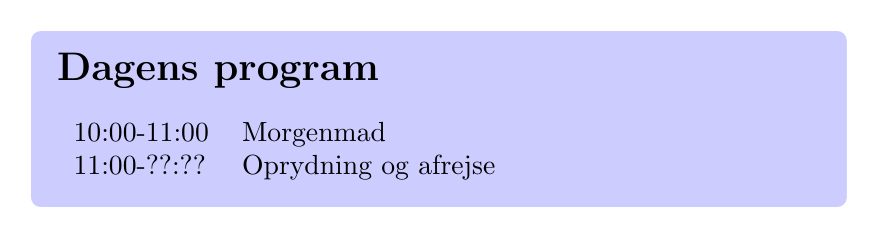
\begin{tikzpicture}
\node [mybox] (box){%
\begin{minipage}{0.80\textwidth}
\vspace{-4mm}\section*{Dagens program}
\begin{tabular}{ll}
10:00-11:00 & Morgenmad \\
11:00-??:?? & Oprydning og afrejse \\
\end{tabular}
\vspace{-4mm}
\end{minipage}
};
\end{tikzpicture}%

\section*{Farvel}
Vi har observeret en signifikant tilvækst i jeres forståelse, med $5\%$ signifikansniveau. Campen har derfor et forventet afkast på $523.817 dkr$ for samfundsøkonomien.

{\flushright\emph{1. co-koordinator, Helene, næsten cand. scient. stat.-oecon.}}

\section*{Farvel}
Jeg elsker jer alle, livet er fedt!!! Syng en sidste sang, og lav et gruppekram!!!

{\flushright\emph{Den ligeste blandt lige, 2. co-koordinator, Morten Agger}}

\section*{Farvel}
Alt for få af jer, har ofret jeres liv for min sag! Jeg er skuffet, så fremadrettet vil kun kloner af ming optages på mine camps. 

{\flushright\emph{Der Führer, Jeres koordinator, Morten Grue Sørensen}}

\end{minipage}
\begin{center}
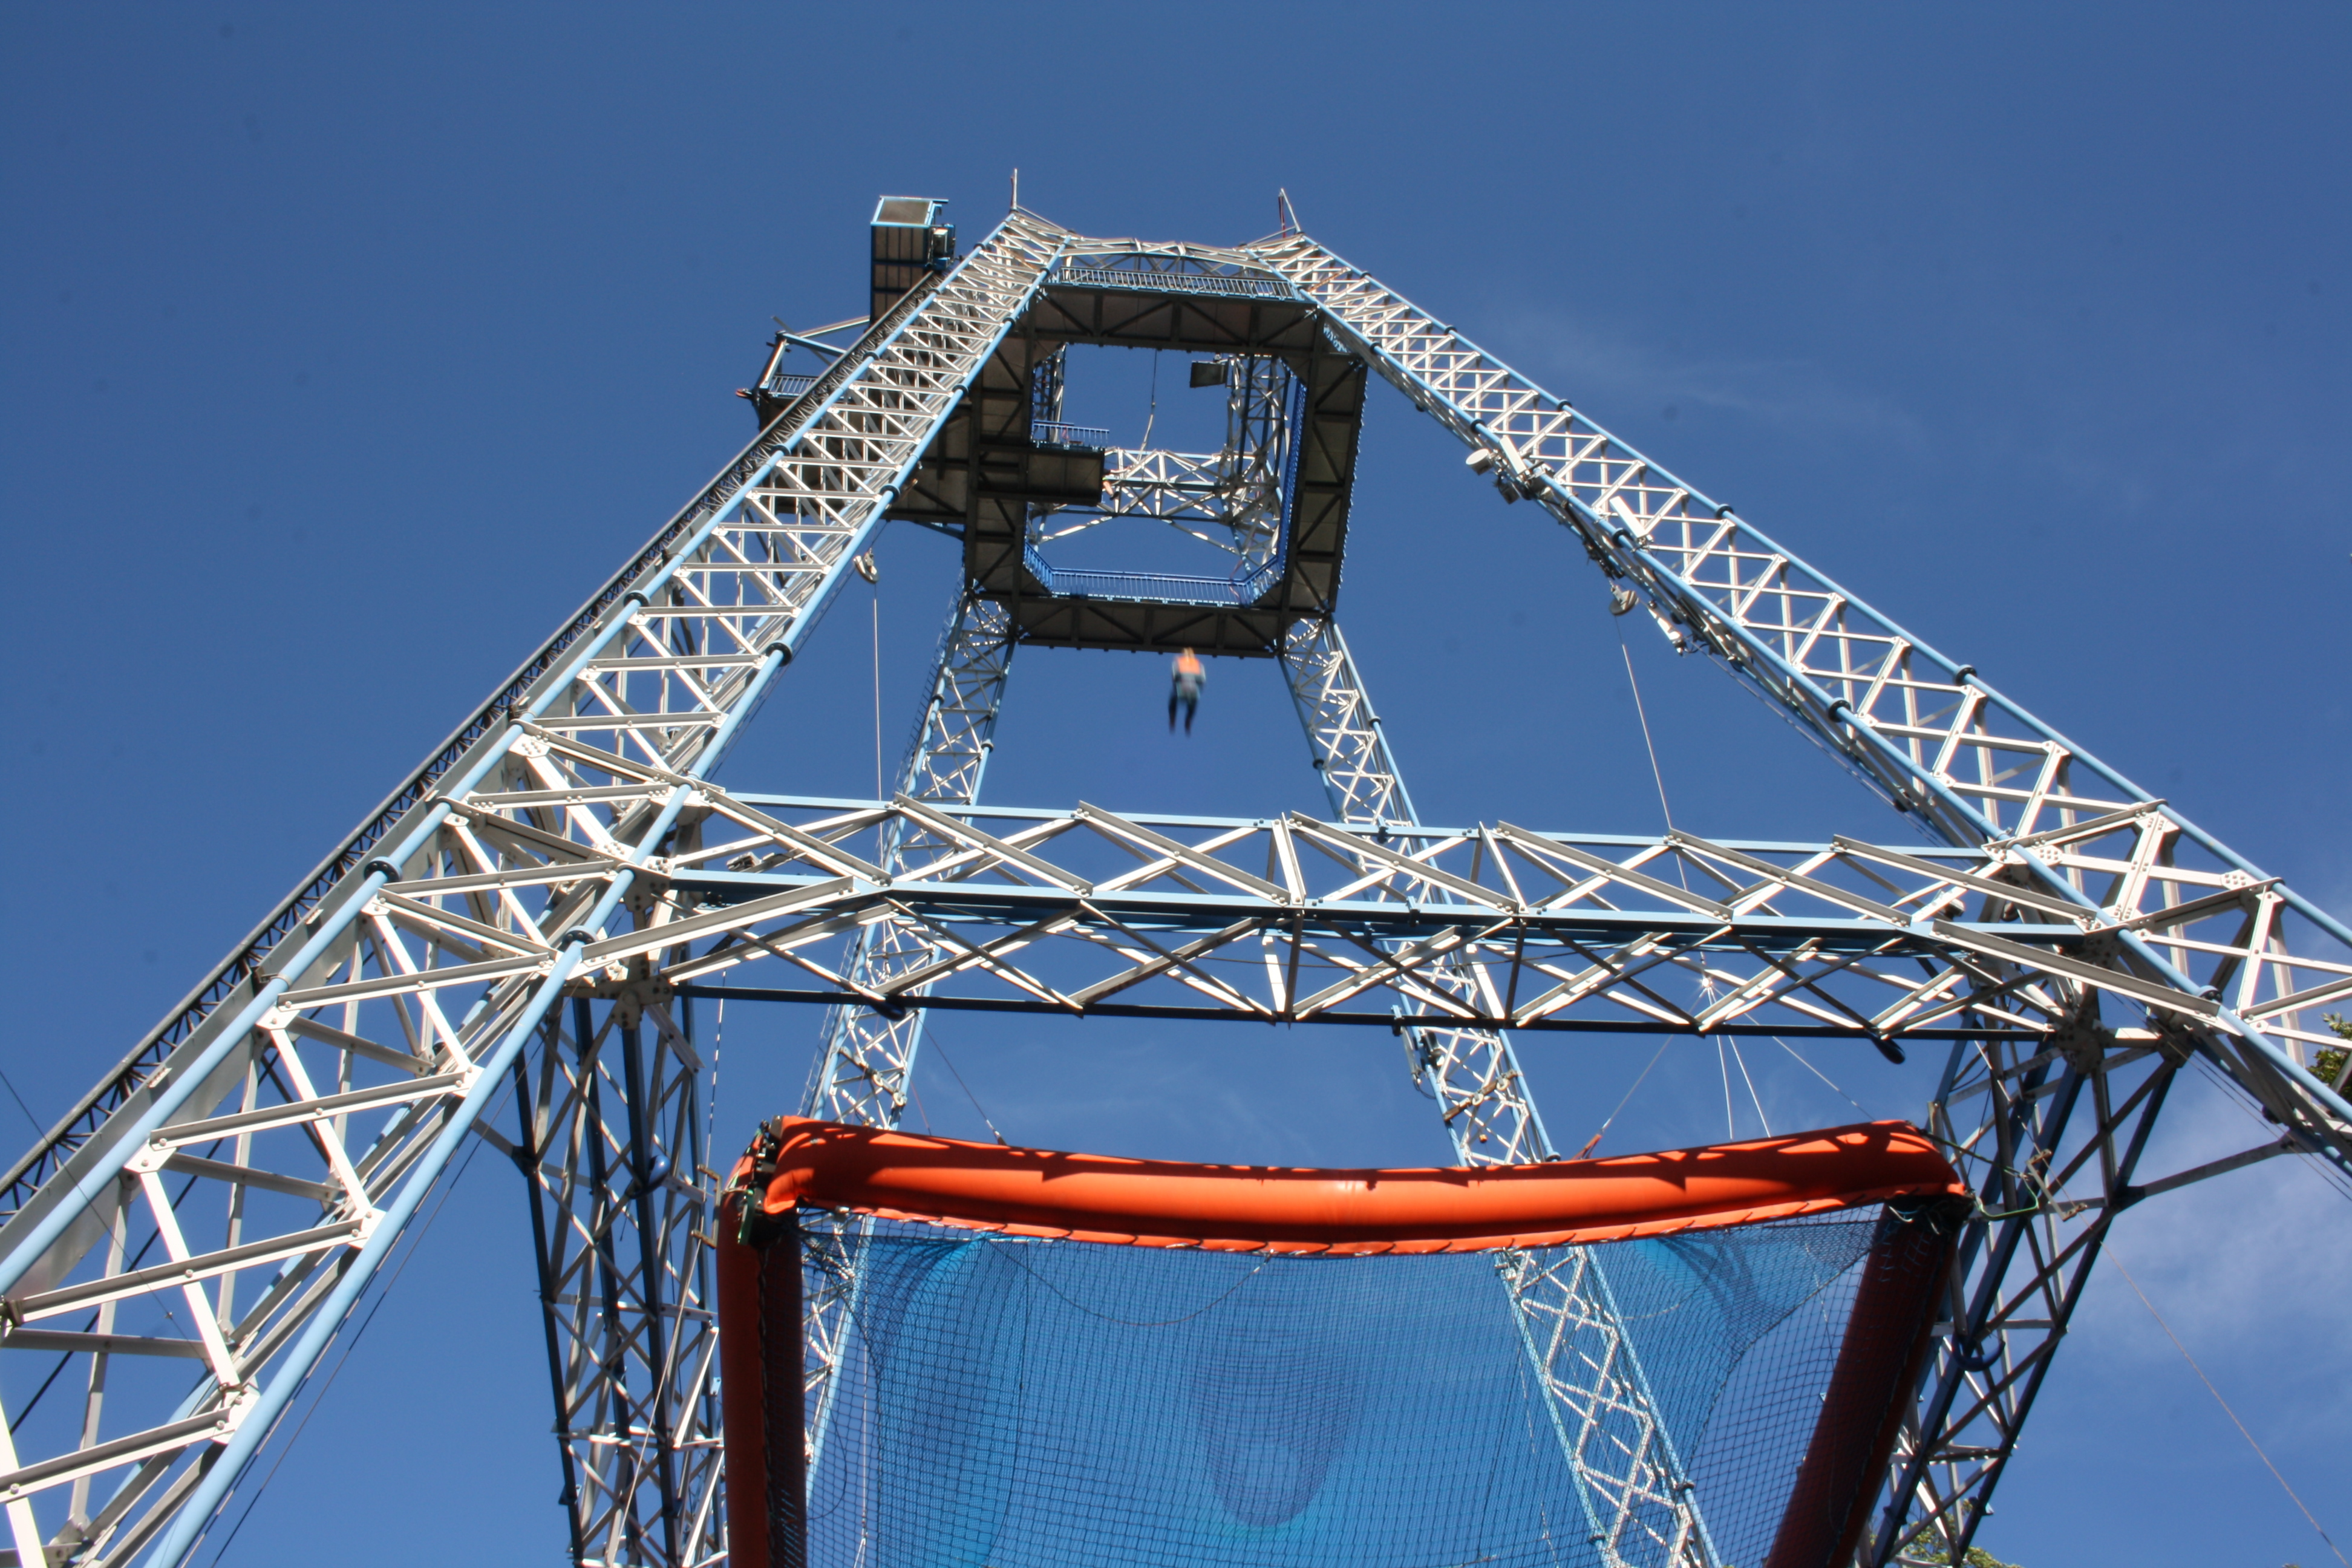
\includegraphics[width=\linewidth]{taarn.jpg}
\end{center}
\end{minipage}
